\documentclass{article}
\usepackage[utf8]{inputenc}

\title{Reply to Examiners}
\author{}
\date{\today}

\usepackage{graphicx}
\usepackage{caption} % to get nicer top captions with tables
\usepackage{subcaption}
\usepackage{amsmath}
\usepackage{placeins}

% to change the colour of text
\usepackage{xcolor}
% to strike through text
\usepackage[normalem]{ulem}

% to help with quoting added material in the revised paper 
\usepackage{quoting}
\newcommand{\say}[1]{%
\begin{quoting}
#1
\end{quoting}
}

\newcommand{\sayold}[1]{%
\say{{\color{olive}#1}}
}

\newcommand{\saydel}[1]{%
\say{{\color{darkgray}\sout{#1}}}
}

\newcommand{\saymod}[1]{%
\say{{\color{blue}#1}}
}

\newcommand{\saynew}[1]{%
\say{{\color{orange}#1}}
}

\newcommand{\reviewcomment}[3]{%
\vspace{4mm}
\textbf{C[$R_{#1}C_{#2}$]:} {\it #3}
\vspace{2mm}
}

\newcommand{\response}[1]{%
{\textbf{R:}} {#1}
}

% Change the default figure/table numbering to avoid confusion with main manuscript
\renewcommand{\figurename}{Fig.}
\renewcommand{\thefigure}{L\arabic{figure}}
\renewcommand{\thetable}{L\arabic{table}} 
\newcommand{\figref}[1]{\figurename~\ref{#1}}
\newcommand{\tabref}[1]{\tablename~\ref{#1}}

\graphicspath{ {./Figures/} }

\usepackage[pdfusetitle,hidelinks]{hyperref}
\bibliographystyle{unsrt}

\begin{document}

\maketitle

In the revised document that we join with this reply, added or modified text is highlighted in \textcolor{red}{red}.
These parts are annotated with $EC_j$ referring to the comment $j$ associated with the amendments in the examiner report, $AC_j$ referring to comment $j$ in the annotated thesis provided, and $SC_j$ referring to a self correction $j$.


%%%
\section{Manuscript Modifications}

The main modifications which we performed to revise our manuscript address these points:
\begin{enumerate}
    \item 1
    \item 2
\end{enumerate}


%%%
\section{Detailed Answer to amendments in examiner report}

We thank you for your careful reading of our manuscript and your helpful comments, including those regarding the strengths and limitations of the study.

\reviewcomment{1}{1}{
 The spectra of the phantoms do not completely follow Hb and HbO2; this should include quantification of this difference and a discussion of how this affects the ability to use these phantoms to test systems.
}

\response{
We agree that this is limitation of our study which could have been better emphasised.
Our discussion now reads: 
\begin{quoting}
Similarly, haemoglobin chromophores could not be utilised in the phantoms due to their oxygen sensitivity which could not be controlled within the spectrophotometer measurement set-up. This led us to rely on stable synthetic dyes instead\textcolor{red}{, which do not perfectly replicate the spectra of oxy and deoxyhaemoglobin. The major dye peaks maxima are approximately 45nm lower than the distinctive haemoglobin peaks which may contribute to different wavelength regions performing differently with these phantoms compared to biological samples}.
\end{quoting}
}

\reviewcomment{1}{2}{The lack of spatial information in the phantoms does not address the ability of systems to determine both spectral and spatial resolution. This can be important in MSI systems as resolution might vary at different wavelengths. Please include this in your discussion.}

\response{
Whilst spatial resolution characterisation is critical to the effective use of HSI systems, this is beyond the scope of this work which aims to evaluate the analytical $StO_2$ methods.
We therefore prefer to refer the reader to publications dedicated to this topic.
This consideration is added to our discussion which now reads: 
\begin{quoting}
    \textcolor{red}{These phantoms are also spatially uniform meaning that, whilst these could be used to determine the performance of these models spatially using hyperspectral imaging systems, other methods would be required to assess spatial resolution of these systems \cite{EdmundOptics2023, Torkildsen2018}.} 
\end{quoting}
}

\reviewcomment{1}{3}{Please add labels to Figure 1(a) to indicate what each part of the phantom shows}

\response{
This figure shows some baseline components used in phantom synthesis and the caption has been revised to clarify this. The revised figure is reproduced as \figref{fig:phantommethods1} in this letter.
\begin{figure}[htb]
    \centering%\revref{1}{3}
    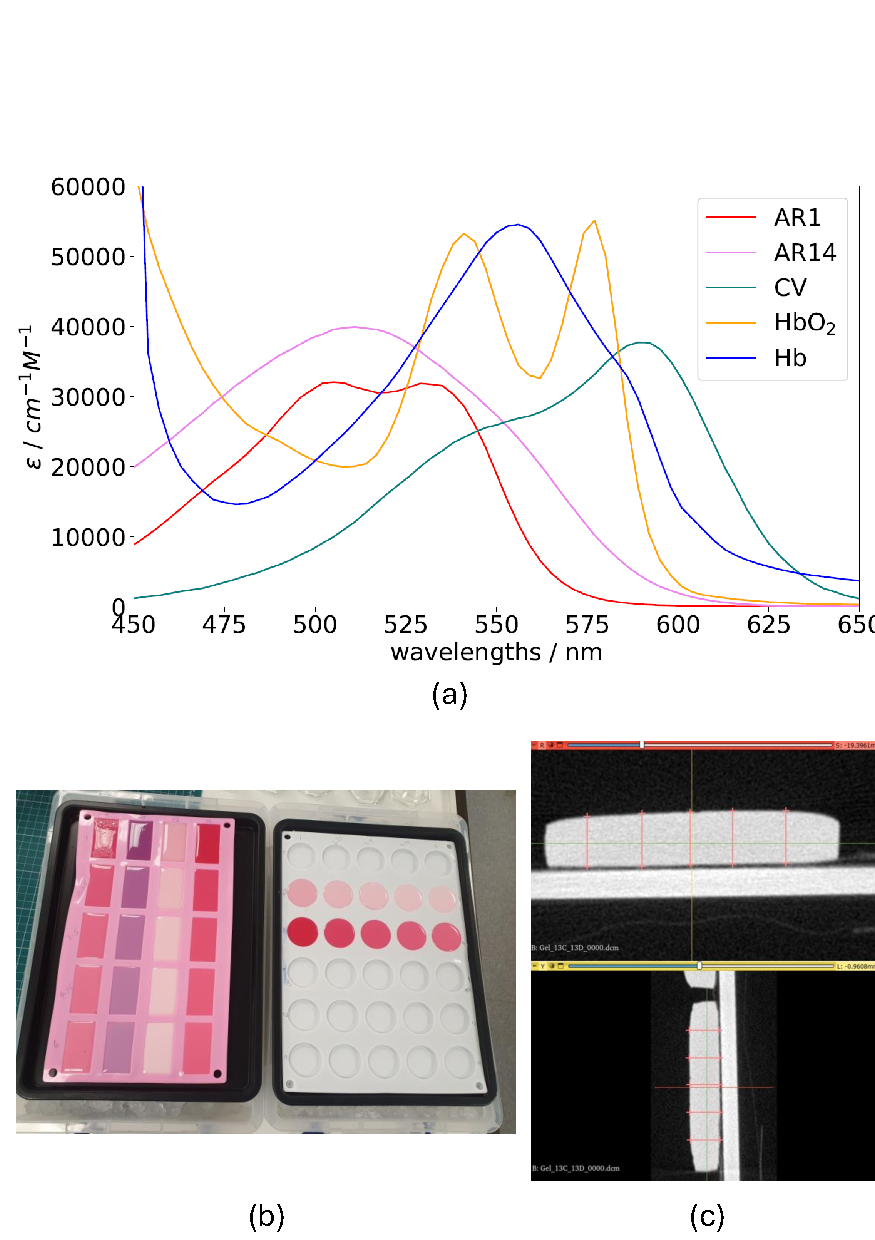
\includegraphics[width=0.8\textwidth]{Figure_1.pdf}
    % \begin{subfigure}{0.6\textwidth}
    %     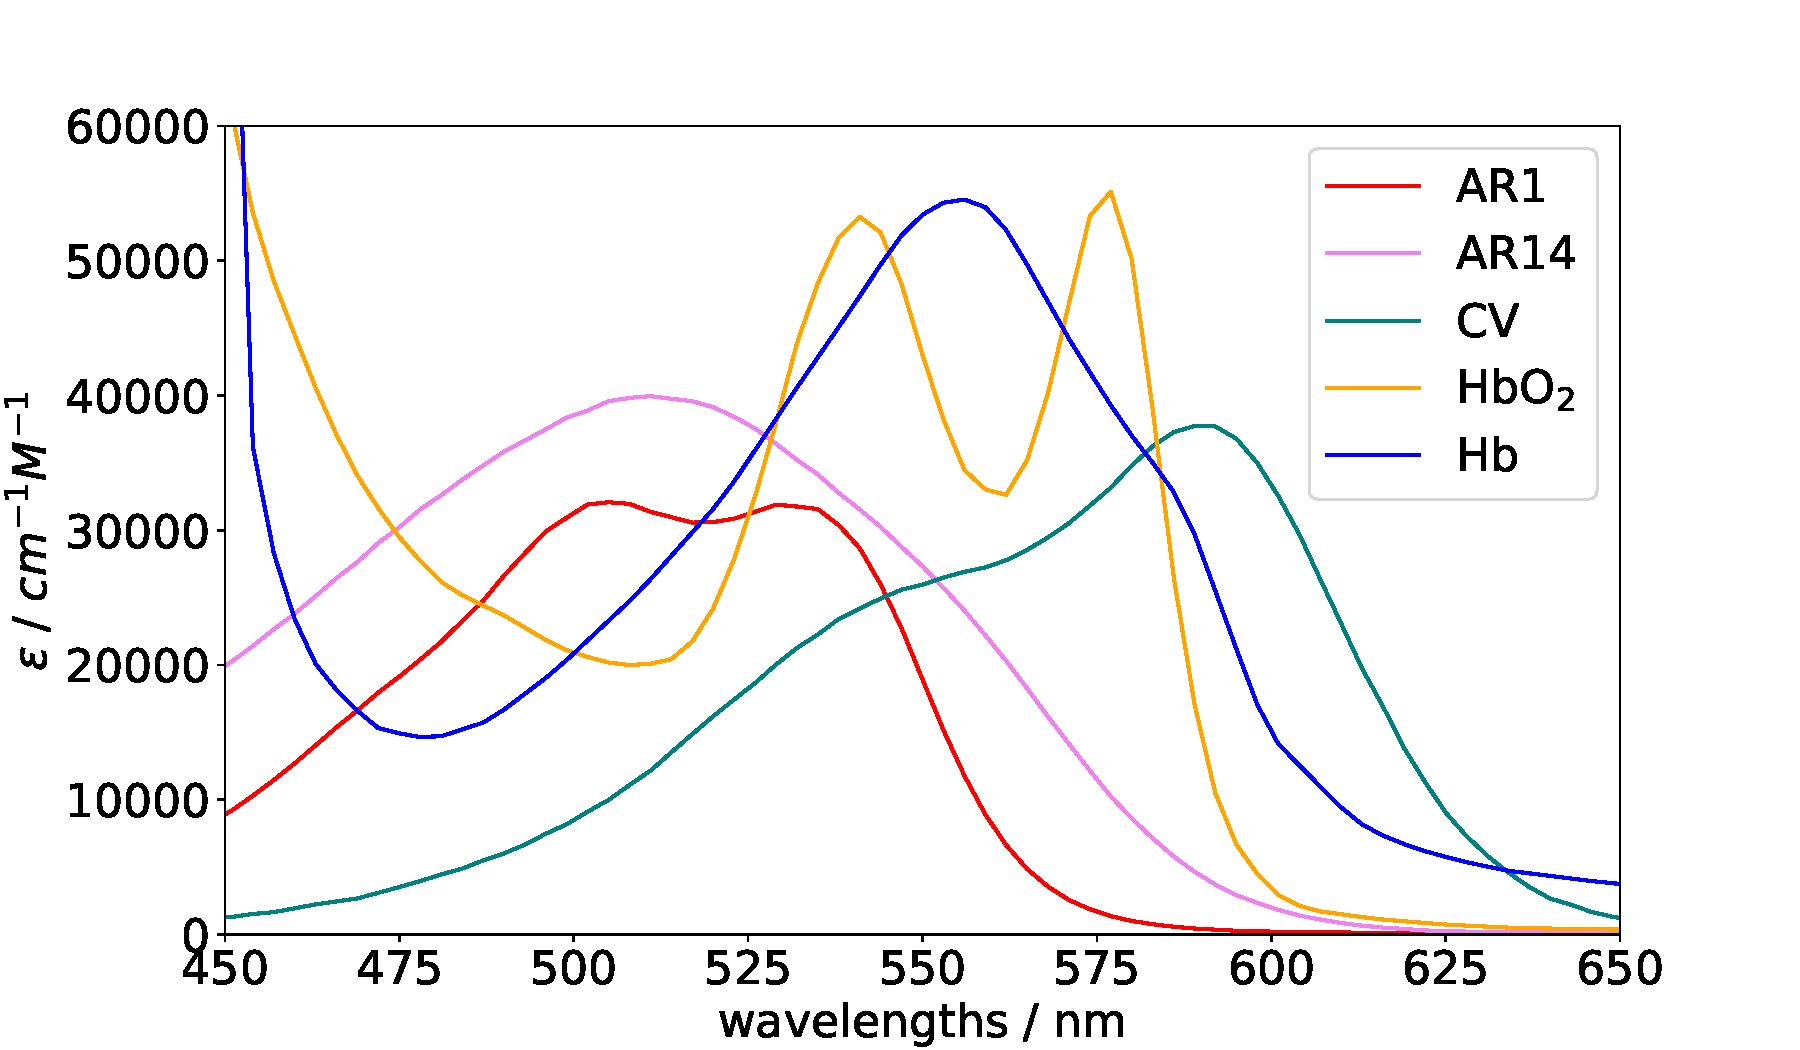
\includegraphics[width=\textwidth]{Figure_1a.pdf}
    %     \caption{}
    %     \label{fig:exteff}
    % \end{subfigure}
    % \hfill
    % \begin{subfigure}{0.44\textwidth}
    %     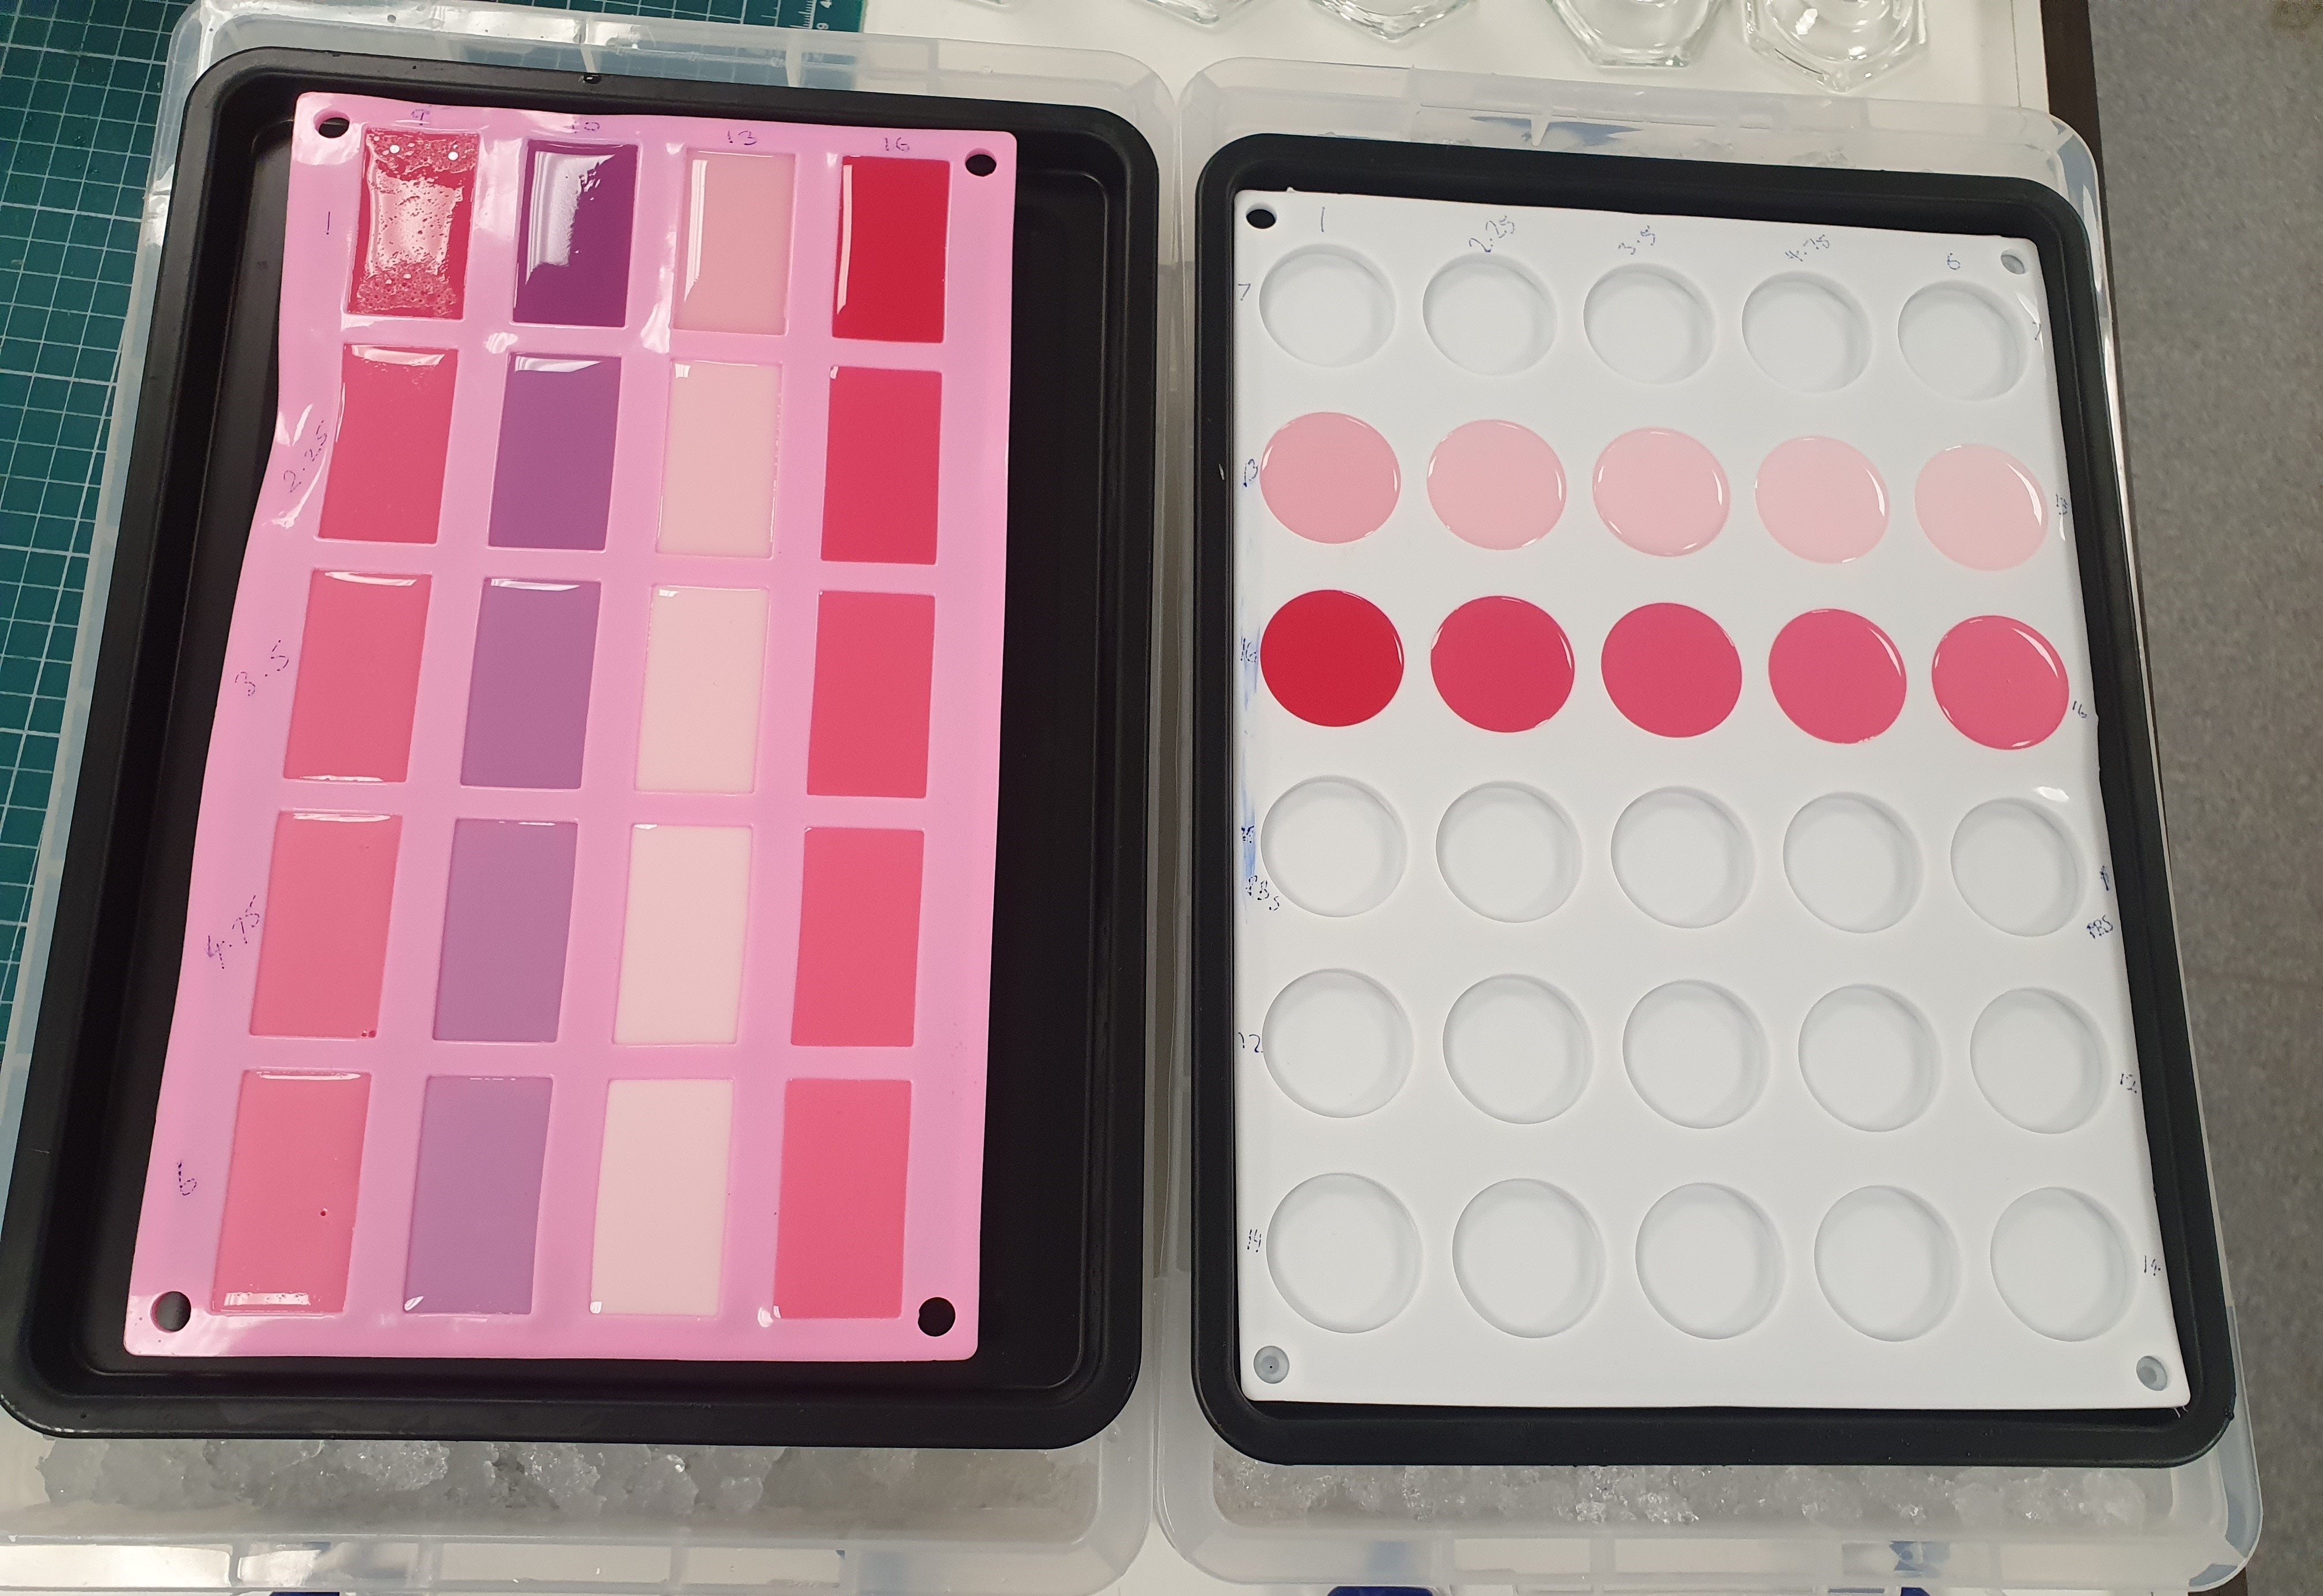
\includegraphics[width=\textwidth]{Figure_1b}
    %     \caption{}
    %     \label{fig:icebath}
    % \end{subfigure}
    % \begin{subfigure}{0.245\textwidth}
    %     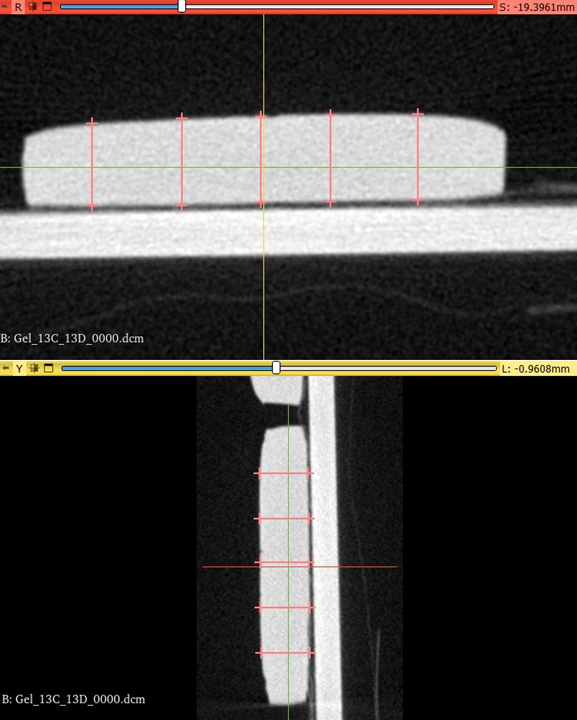
\includegraphics[width=\textwidth]{Figure_1c}
    %     \caption{}
    %     \label{fig:DICOM_Eg}
    % \end{subfigure}
    \caption{Figure regarding phantom development. 
    \textbf{(a)}
    Effective extinction coefficients of acid red 1 (AR1), acid red 14 (AR14), and crystal violet (CV) dyes \textcolor{red}{(used to synthesis gelatin-based phantoms)} are displayed with the extinction coefficients of oxygenated (HbO$_2$) and deoxygenated haemoglobin (Hb) \textcolor{red}{(key tissue chromophores)}.
    \textbf{(b)}
    Image of 1cm depth (left) and 5mm depth (right) phantoms setting in ice bath.
    \textcolor{red}{\textbf{(c)}
    An example of a CT scan acquired for the purpose of measuring thickness of a tissue phantom is shown with
    %the
    10 digital measurements (mean=6.11mm)%
    %taken whose mean is calculated to be 6.11mm
    }.}
    \label{fig:phantommethods1}%\revref{1}{5}
\end{figure}
}
\FloatBarrier

\reviewcomment{1}{4}{Table 1 is confusing; perhaps use percentages instead of ratios, as these are more uniform.}

\response{
Please find the revised table reproduced as \tabref{tb:phantomratios} in this letter. This can be found as Table 1 in the main manuscript.
\begin{quoting}
    \begin{table}[ht!]
    \centering
    \caption{Table displaying the \textcolor{red}{percentage of each }dye [acid red 1 (AR1), acid red 14 (AR14), crystal violet (CV)] a used for each dye configuration alongside the total dye scaled concentration in arbitrary units.}
    \color{red}
    \begin{tabular}{|c|c|c|c|}
        \hline
        Total dye scaled concentration & \multicolumn{3}{|c|}{Dye \textcolor{red}{percentage (\%)}} \\
        (arbitrary units) & AR1 & AR14 & CV \\
        \hline
        1 & 50 & 50 & 0 \\
        1 & 50 & 25 & 25 \\
        1 & 25 & 25 & 50 \\
        10 & 100 & 0 & 0 \\
        10 & 75 & 25 & 0 \\
        10 & 50 & 50 & 0 \\
        10 & 25 & 75 & 0 \\
        10 & 0 & 100 & 0 \\
        10 & 25 & 50 & 25 \\
        10 & 50 & 25 & 25 \\
        10 & 25 & 25 & 50 \\
        20 & 50 & 50 & 0 \\
        20 & 50 & 25 & 25 \\
        20 & 25 & 25 & 50 \\
        \hline
    \end{tabular}
    \label{tb:phantomratios}
\end{table}
\end{quoting}
}

\reviewcomment{1}{5}{I’m not sure what the CT scan adds to the paper. It should be better addressed.}

\response{
We agree that the rationale for using a CT scan is could have been strengthened. This has now been done in Section 2.2.2 of the revised manuscript which we reproduce here.
\begin{quoting}
    In order to obtain accurate optical properties from IAD a highly accurate sample depth must be provided. \textcolor{red}{The standard measurement technique using dial calipers is not suitable in this case due to the highly compressible nature of the gelatin-based phantoms.
    A non-contact measurement method is therefore chosen. A} CT scan is taken of each phantom using a Small Animal Radiotherapy System (SmART+, precision X-ray). A mean of 10 digital measurements is used for each phantom and an example of these measurements is shown in Figure 1c [Note: \figref{fig:phantommethods1}c in this letter].
\end{quoting}
The caption for Figure 1c has also been amended as shown in \figref{fig:phantommethods1} c in this letter. 
%\begin{figure}[htb]
%    \centering%\revref{1}{3}
%    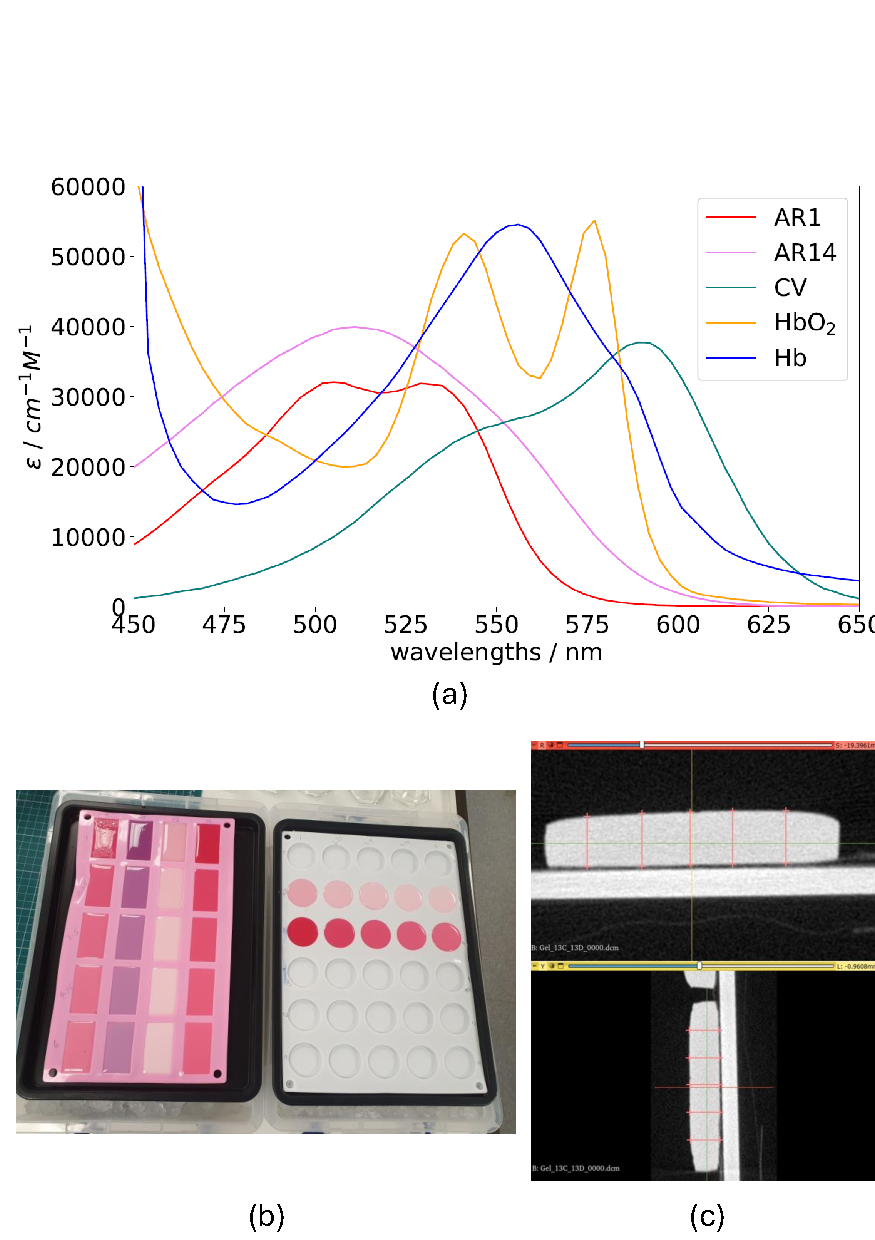
\includegraphics[width=0.5\textwidth]{Figure_1.pdf}
    % \begin{subfigure}{0.6\textwidth}
    %     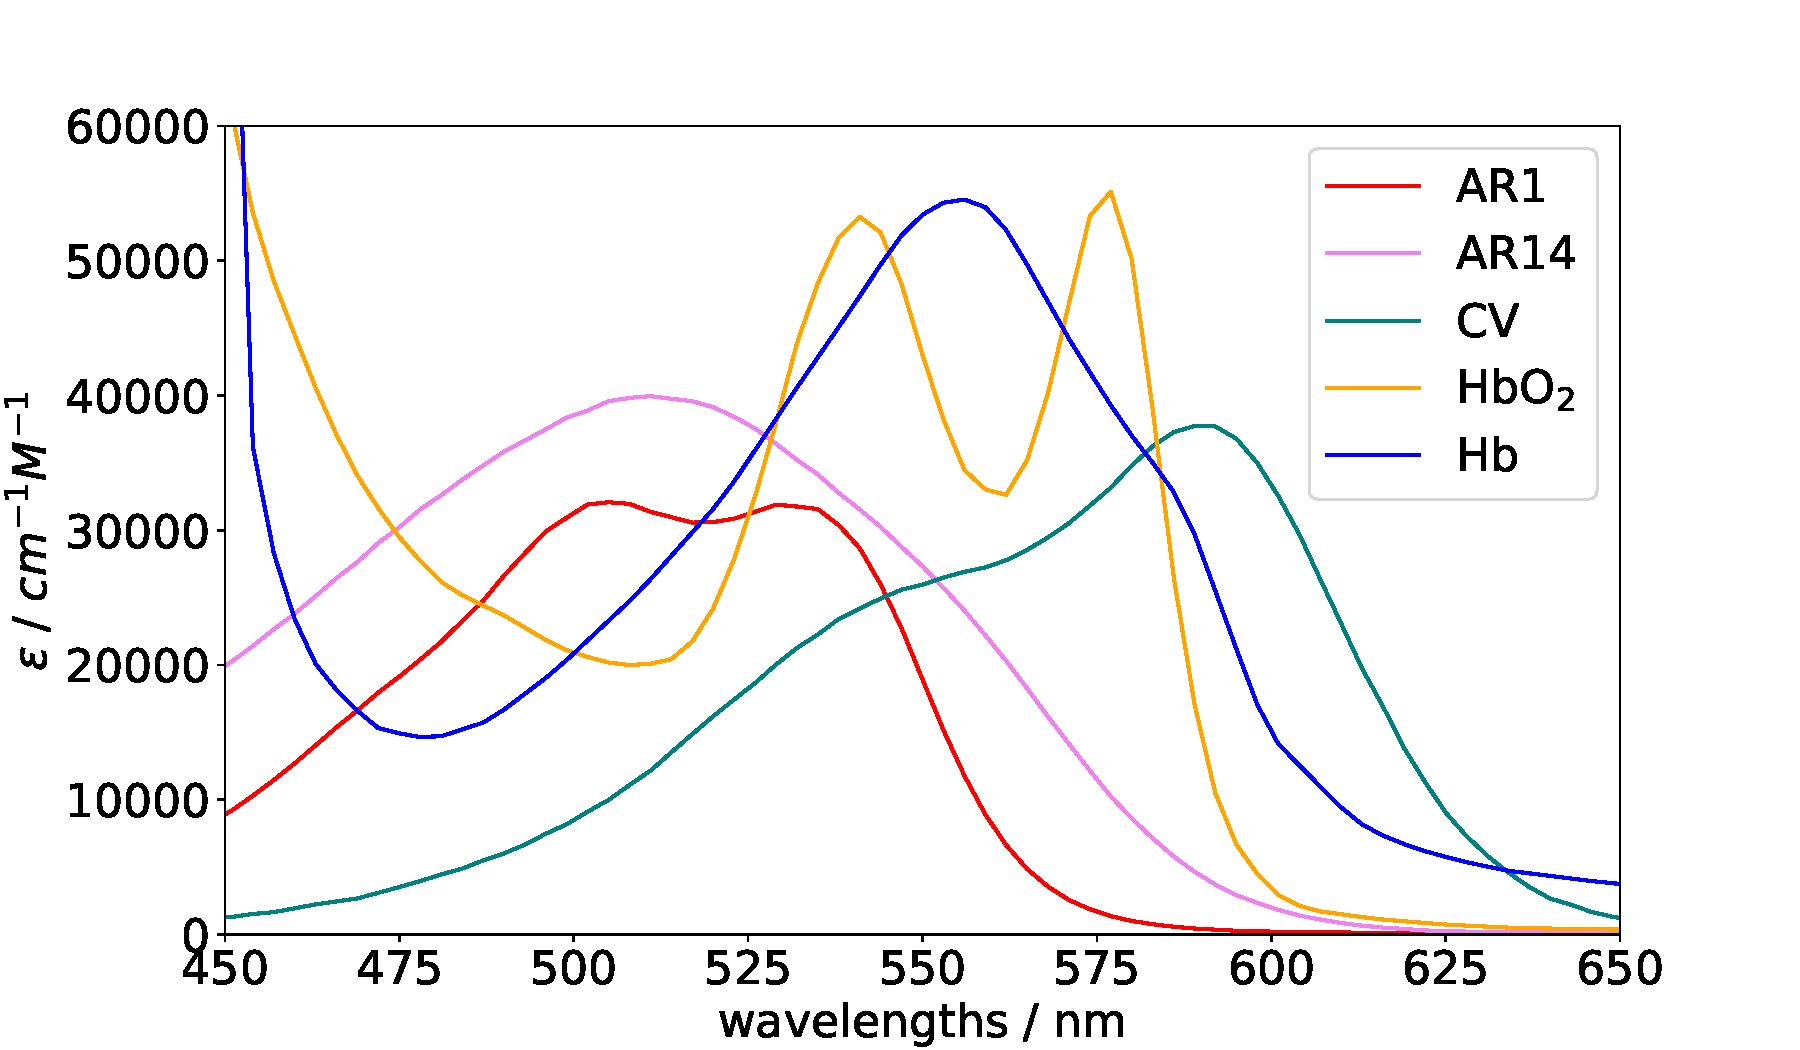
\includegraphics[width=\textwidth]{Figure_1a.pdf}
    %     \caption{}
    %     \label{fig:exteff}
    % \end{subfigure}
    % \hfill
    % \begin{subfigure}{0.44\textwidth}
    %     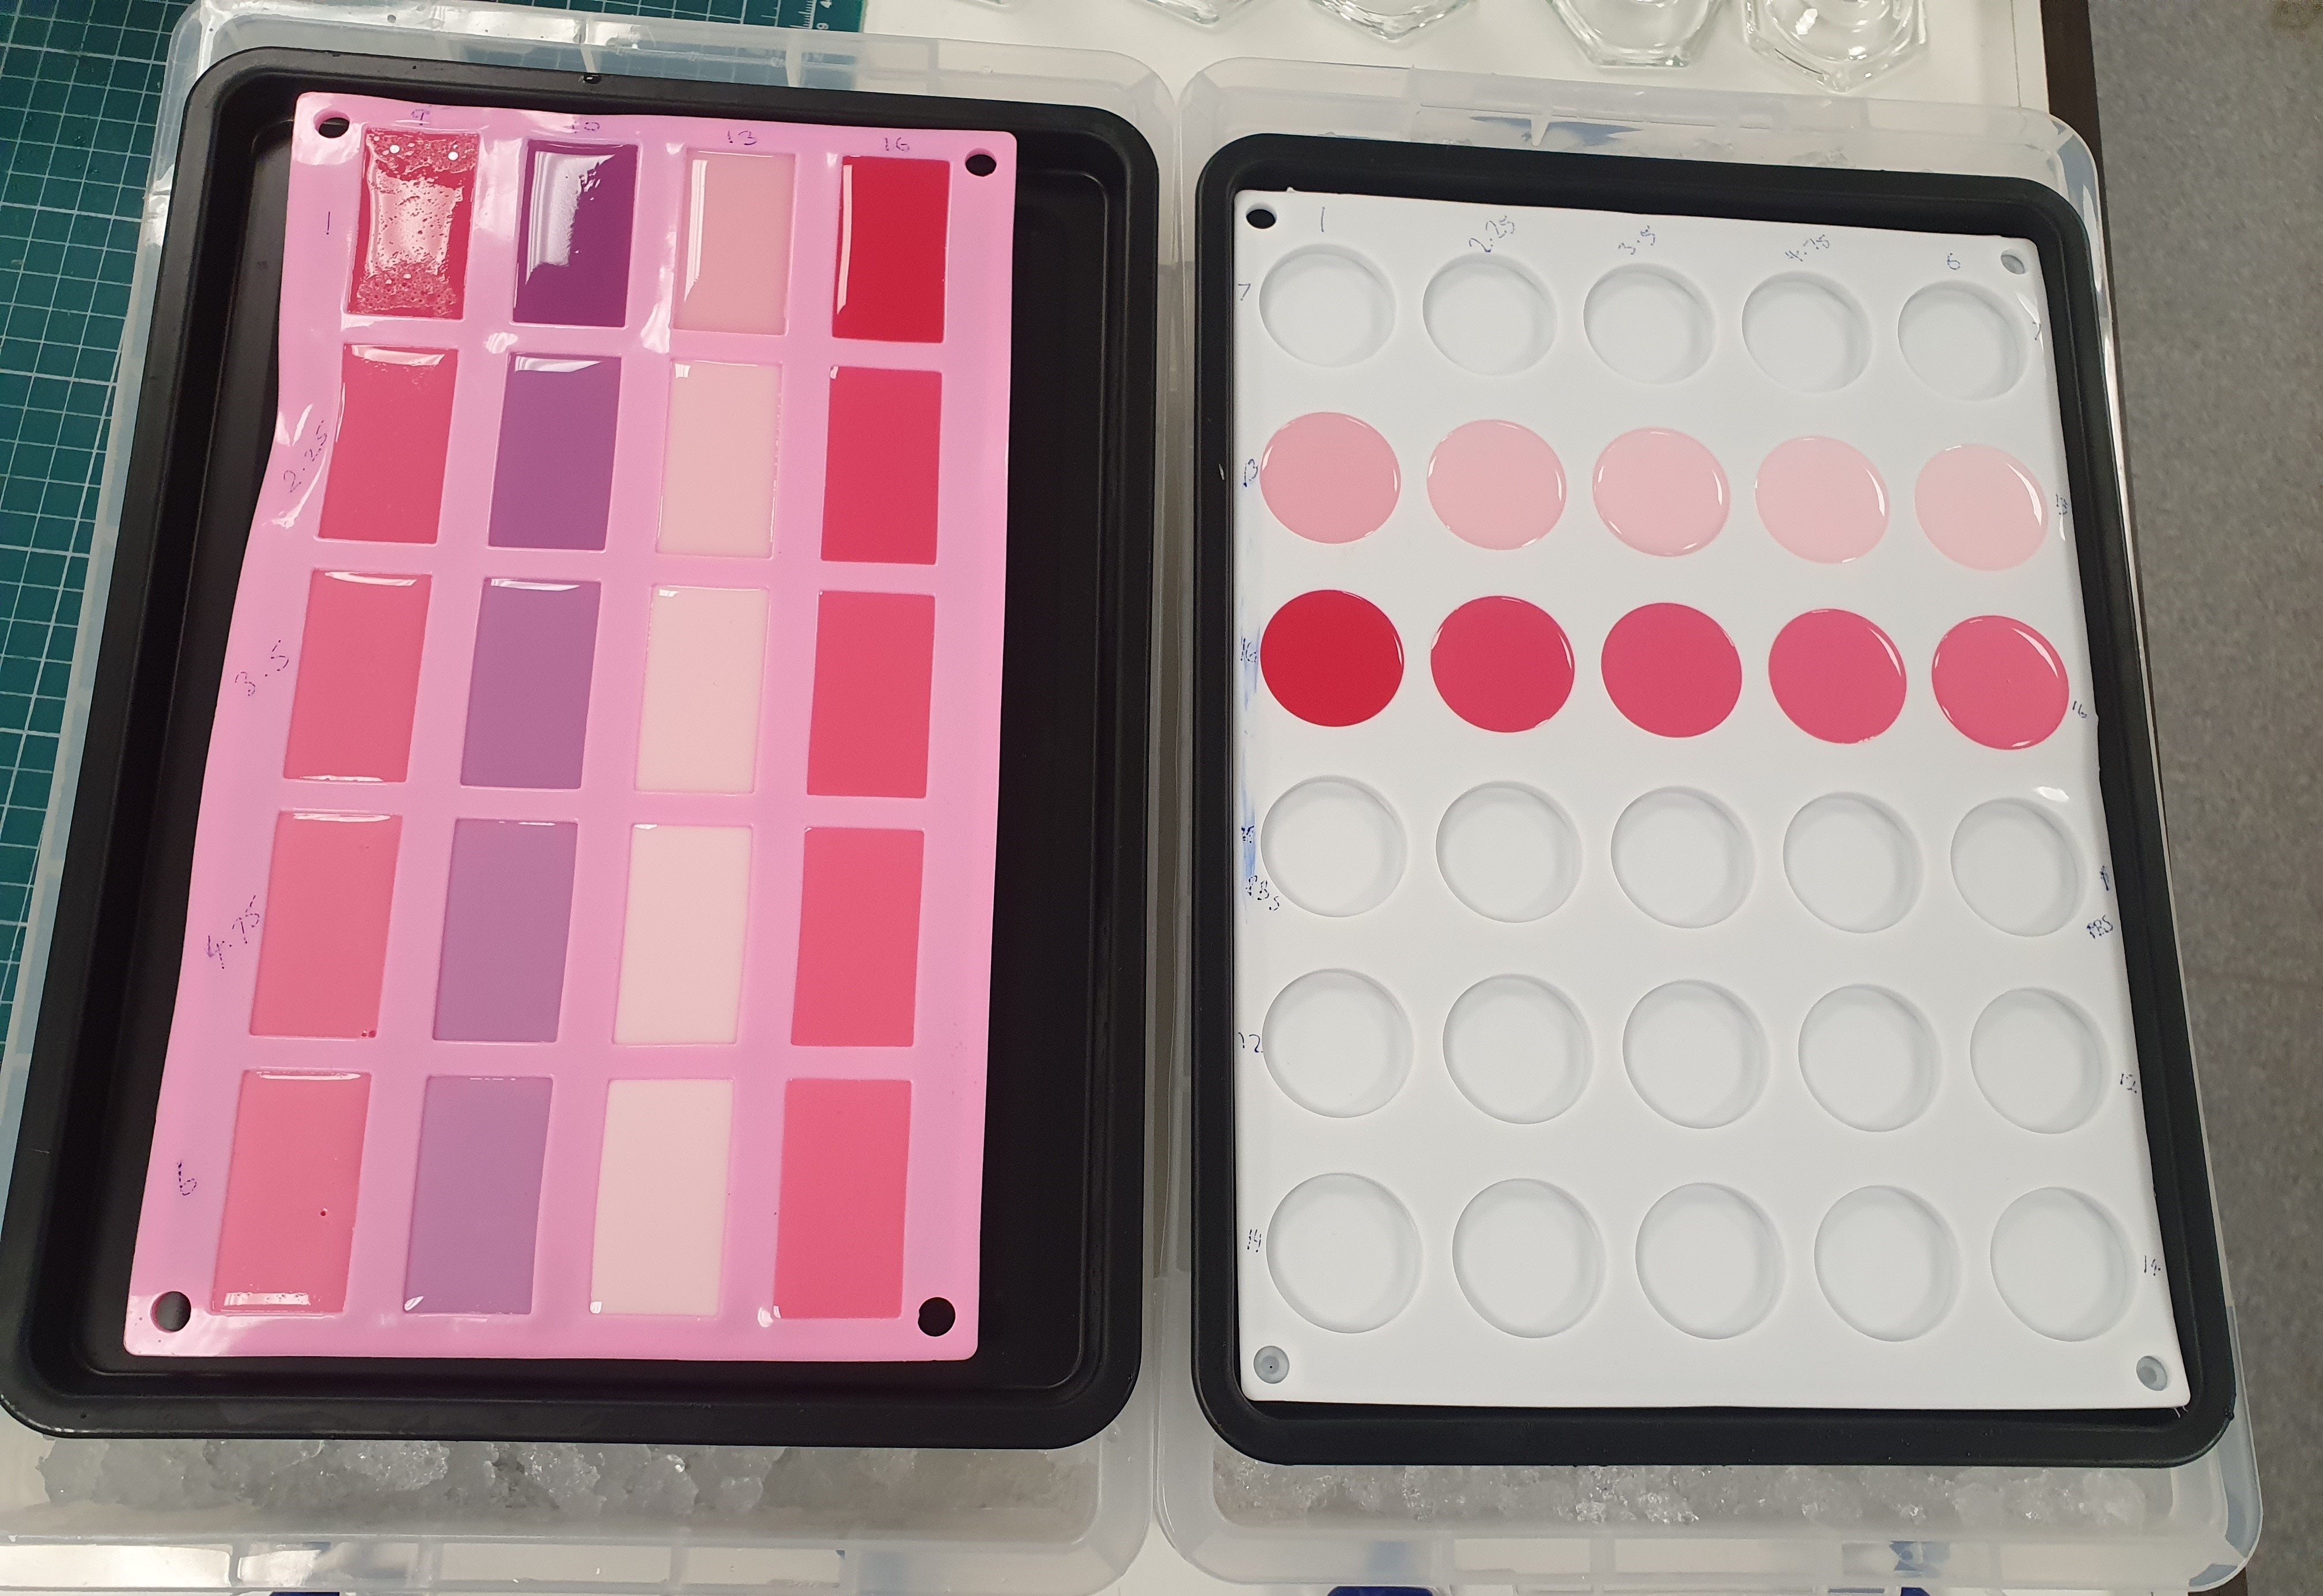
\includegraphics[width=\textwidth]{Figure_1b}
    %     \caption{}
    %     \label{fig:icebath}
    % \end{subfigure}
    % \begin{subfigure}{0.245\textwidth}
    %     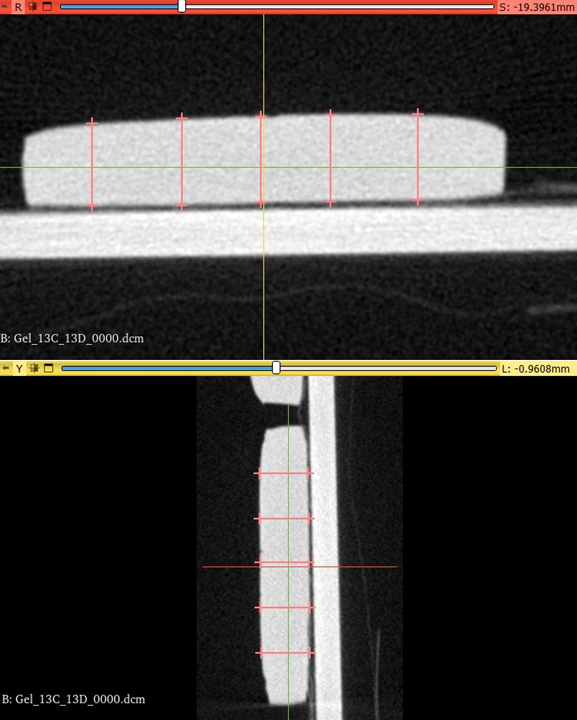
\includegraphics[width=\textwidth]{Figure_1c}
    %     \caption{}
    %     \label{fig:DICOM_Eg}
    % \end{subfigure}
%    \caption{Figure regarding phantom development. Effective extinction coefficients of acid red 1 (AR1), acid red 14 (AR14), and crystal violet (CV) dyes (used to synthesis gelatin-based phantoms) are displayed with the extinction coefficients of oxygenated (HbO$_2$) and deoxygenated haemoglobin (Hb) (key tissue chromophores) (a). Image of 1cm depth (left) and 5mm depth (right) phantoms setting in ice bath (b). \textcolor{red}{An example of a CT scan acquired for the purpose of measuring thickness of a tissue phantom is shown with the 10 digital measurements taken whose mean is calculated to be 6.11mm} (c).}
%    \label{fig:phantommethods2}%\revref{1}{5}
%\end{figure}
}
%\FloatBarrier

\reviewcomment{1}{6}{Finally, please discuss the downsides/trade-offs of the phantoms.}

\response{
This has been added to the discussion also in line with our answers to the previous comments. The revised text is reproduced below. 
\begin{quoting}
    Firstly, whilst every effort was made to synthesise optical phantoms resembling biological tissue, measurements of true biological tissue could not be used for this work due to a lack of reliable ground truth parameters in tissue.
%, alongside challenges in integration to the surgical work flow since the surgical procedure cannot continue during the in-vivo data capture process. 
Similarly, haemoglobin chromophores could not be utilised in the phantoms due to their oxygen sensitivity which could not be controlled within the spectrophotometer measurement set-up. This led us to rely on stable synthetic dyes instead\textcolor{red}{, which do not perfectly replicate the spectra of oxy and deoxyhaemoglobin. The major dye peaks maxima are approximately 45nm lower than the distinctive haemoglobin peaks which may contribute to different wavelength regions performing differently with these phantoms compared to biological samples}. \textcolor{red}{The factors chosen to allow approximately equal impact from each dye were chosen to ease synthesis and should be optimised. Since these factors are incorporated in both synthesis and analysis, it is believed that these do not impact the conclusions of this study.}\textcolor{red}{The difference in extinction coefficient found when measuring each dye in gelatin compared to aqueous solution is not fully understood and requires further study.}\textcolor{red}{These phantoms are also spatially uniform meaning that, whilst these could be used to determine the performance of these models spatially using hyperspectral imaging systems, other methods would be required to assess spatial resolution of these systems \cite{EdmundOptics2023, Torkildsen2018}.} Secondly, the shift in absorbance of the third chromophore made it difficult to model thereby limiting the investigation of the impact of additional chromophores.
%
Thirdly, whilst the IAD method produces results similar to our ground truth, there remain some differences between IAD output and the expected ground truth.
This could impact the quality of the intralipid scattering model used in this work.
\end{quoting}
}

%%%
\section{Amendments addressed from annotated manuscript}

Thank you for your careful reading of this manuscript and your helpful comments. I have compiled these in the following table with associated changes being clearly indicated in the revised document. 

\begin{table}
    \centering
    \begin{tabular}{|p{1.5cm}|p{2cm}|p{7.5cm}|}
        \hline
        Number & Page in annotated manuscript & Comment \\
        \hline
        1 & 5 & Correct formating of StO2 to $StO_2$ \\
        2 & 5 & State how many neurosurgical cases were investigated \\
        3 & 9 & Update list of publications to reflect changes since submission \\
        4 & 34 & State application need of existing adjuncts \\
        5 & 37 & Add percentage symbol to $StO_2$ equation \\
        6 & 38 & State only visible range displayed in Figure 1.3 caption \\
        7 & 38 & Clarify that "lack specificity" refers to cerebral oximetry techniques not being able to distinguish between tissues \\
        8 & 38 & Include distinction between absolute and relative $StO_2$ changes \\
        9 & 39 & Clarify that it is common to take measurements within the range of 400-1000~nm, however not all measurements span the full range \\
        10 & 40 & Clarify how use of isosbestic point relates to Equation 1.5 \\
        11 & 40 & Clarify that not all pulse oximetry uses this technique \\
        12 & 40 & Add advantages of using multiple wavelengths \\
        13 & 40 & Clarify what the derivative of the spectrum is taken with respect to \\
        14 & 42 & Specify type of algorithms used for tissue differentiation \\
        15 & 43 & Explain how optical energy is converted to thermal energy \\ 
        16 & 43 & Correct to reflect that quantitative $StO_2$ can be obtained from photoacoustic imaging \\
        17 & 44 & State problem with introducing more optical components \\
        18 & 51, 77, 105, 123 & Add footnote to define initials in foreward \\
        19 & 52 & Clarify why white balancing is required \\
        20 & 52 & Define ratiometric \\
        21 & 53 & Define absolute vs relative scale \\
        22 & 54 & \textcolor{red}{State optical power of light sources} \\
        23 & 54 & State alternatives to bilinear interpolation \\
        24 & 59 & Detail how frequently ruler swipe would need to be repeated in theatre \\
        25 & 60, 74 & How stable are the light sources and could light source stability be an issue? \\
        26 & 62 & Clarify what kind of imperfections can occur in video processing \\
        27 & 73 & Move section to conclusion \\
        28 & 75 & Explain exposure settings \\
        29 & 76 & Explain how this affects $StO_2$ calculation and link to the aimed $StO_2$ resolution \\
        30 & 82, 110, 164 & \textcolor{red}{State computer system used and time taken to generate simulations} \\
        31 & 83 & Expand on correction factors \\
        32 & 83, 85 & Indicate $\mu_a$ values from each phantom configuration \\
        33 & 83 & Clarify that intralipid only affects the scattering component \\
        34 & 83 & Clarify that variety of composition parameters chosen are detailed in previous paragraphs \\
        35 & 84 & Clarify in what way the dyes mimic haemoglobin \\
        36 & 85 & Why was a 5~mm depth chosen? \\
        37 & 87 & Clarify that the reference spectra are those generated from the methods detailed in previous sections \\
        38 & 91, 94, 96 & Link large errors in BL results to the scale of $mu_a$ differences being resolved \\
        39 & 93, 97 & Discuss CV-intralipid conjugation \\
        40 & 93 & Explain importance of shift in extinction coefficients \\
        41 & 94 & Suggest why phantom spectra fit poorly after 575~nm \\
        42 & 95 & Clearly indicate where figure is being discussed in text \\
        43 & 98 & Clearly indicate where table is being discussed in text \\ 
        44 & 99 & Detail which prior knowledge is required for phantoms \\
        45 & 99 & Clarify why couldn't use haemoglobin in phantoms even when knowing the extinction coefficients \\
        46 & 100 & \textcolor{red}{Reference explanation of SFDI in the introduction} \\
        47 & 100 & Future work should include phantoms using haemoglobin \\
        48 & 107 & Give examples of other chromophores accounted for by $\mu_{a, back}$ in skin \\
        49 & 107 & Why is $StO_2$ bounded to 20\% instead of 0\% \\
        50 & 110 & Explain why two-layer model results are worse than single-layer in results as well as discussion \\
        51 & 115, 116 & Suggest why NIST data results are so different from literature and why $StO_2$ range is so broad \\
        52 & 115 & \textcolor{red}{Plot $StO_2$ against $f_{mel}$} \\
        53 & 116 & Rephrase why $StO_2$ is chosen to visualise failure region \\
        54 & 117 & Rephrase why two-layer model could be considered for brain \\
        55 & 123 & Clarify if trying to incorporate system parameters into simulation results \\
        56 & 146 & Give types of noise that require reduction \\
        57 & 147 & Explain cross-talk effects here \\
        58 & 147 & Expand on how chose to shift extinction coefficients by 3~nm \\
        59 & 148 & Detail how else you could evaluate HELICoiD results without ground truth \\
        60 & 148 & Emphasise impact of slow computational time as a limitation \\
        61 & 165 & \textcolor{red}{Give more details on optimising wavelengths and number of bands in future} \\
        62 & 165 & \textcolor{red}{Give more details on inverse Monte Carlo} \\
        63 & 165 & \textcolor{red}{Why mentioning that lipids have limited human measurements?} \\
        \hline
    \end{tabular}
\end{table}


\section{Self corrections}
On reflection and based on discussion during the viva voce examination, I have identified some minor errors in the original manuscript and have corrected these in this revision. Please find these documented in the following table with all associated changes clearly indicated in the revised document. 
\begin{table}
    \centering
    \begin{tabular}{|p{1.5cm}|p{2cm}|p{7.5cm}|}
        \hline
        Number & Page in annotated manuscript & Comment \\
        \hline
        1 & 76 & Did not collect own clinical HSI data in the end so remove that sentence \\
        2 & 81 & Correct denominator in Yudovsky 2009 equation \\ 
        3 & 95, 97 & Remove factor of 100 from relative reflectance y-axes in Figures 3.7 and 3.8 \\
        4 & 59 & Include figure to demonstrate ruler moving across FOV \\
        5 & 58, 62 & Both the number of bands and noise are denoted by $N$ so change noise to $X$ to avoid confusion \\ 
        6 & 58 & Change the word intuitive as not quite right \\
        7 & 63, 88, 108 & Provide parameters for least squares fitting routines used \\ 
        8 & 83 & Specify the conversion between $f_{blood}$ \% and $moldm^{-3}$ \\
        9 & 81 & Clarify that the extensive and simplified Yudovsky models behave similarly \\
        10 & 115, 121 & Reduce number of example spectra for NIST dataset to make graphs clearer \\
        11 & 124, 149 & Clarify that the optical properties of other system components should be included in the camera simulation \\ 
        12 & 127 & Clarify that the wavelength shift of haemoglobin extinction coefficients is a simplistic approach and other transformations could be necessary \\
        13 & 113, 119 & Plot errors in $StO_2$ against $f_{mel}$ to demonstrate correlation \\
        \hline
    \end{tabular}
\end{table}

\bibliography{Paper2}
\end{document}

